\documentclass[10pt]{article}\usepackage[margin=.55in]{geometry}\usepackage[T1]{fontenc}\usepackage{graphicx}\setlength{\parindent}{0pt}\setlength{\parskip}{4pt}\sloppy\begin{document}{\large Explicit target-information certificates}\par Exact offline validation, 2 November 2026. All 64 retained native relation systems have directly checked certificates. Thirty-nine have a row combination isolating scalar 2, matching every retained returned scalar. Twenty-five have a checked affine solution and target-varying null direction, matching every retained capped control. All 6,900 source-bound rows are edge relations.\par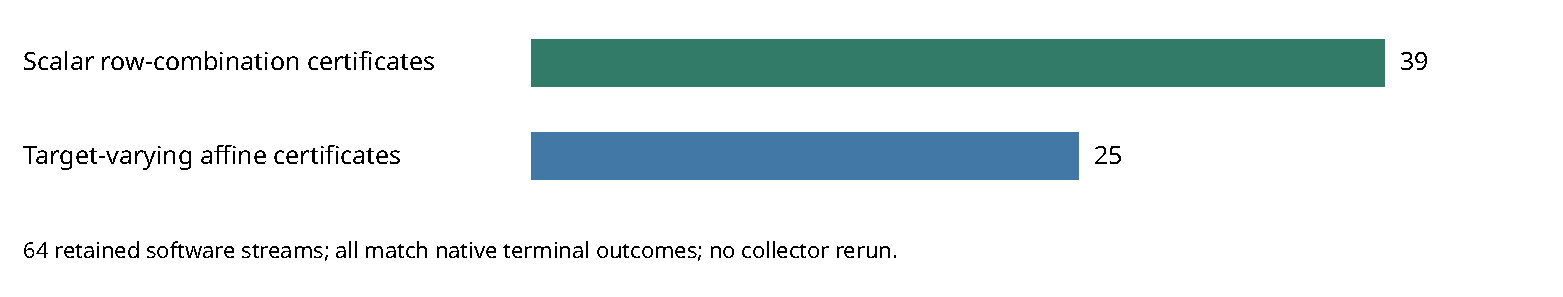
\includegraphics[width=.9\linewidth]{diagram.pdf}\par Convention. Each row is [U,-b,-a], representing U*x-b*k-a=0 over the prime field of order 34147. Node0 is known zero and omitted. Repeated node contributions are added modulo the prime. A separate row extractor rechecks the full row list and event origins against the hashed native streams. The inputs remain the same 64 software traces on the p=739 target 2G instance, not 64 distinct cohort targets.

Determined certificate. The stored weights form a linear combination of rows equal to [0,1,-k]. Taking that same combination of the equations gives k-k\_recorded=0. Each determined certificate also includes a particular solution. The direct checker verifies every equation on that solution as well as the weighted sums, establishing consistency and uniqueness together. It uses no elimination, inverses or native signed-graph code. Each of the 39 resulting scalar values equals the native terminal value already verified on the source curve in the prior packet.

Undetermined certificate. Each stored point z0 solves the equations with target coordinate 0. Each stored direction d has target coordinate 1 and annihilates every variable coefficient row. Hence z0+t*d solves every recorded equation and has target coordinate t, for every field element t. This statement concerns the information in the recorded linear system; geometric restrictions on nuisance variables are outside this certificate.

Validation. The producer uses separately written Gaussian elimination with tracked row combinations. A fresh checker process verified all 64 certificates and their source rows using direct modular sums only. Four synthetic systems cover determined, undetermined, inconsistent and empty cases; their corrupted certificates reject. Five mutations of actual artifacts also reject: scalar, row weight, particular solution, null direction and source row. A valid scalar-isolating combination on an inconsistent synthetic system also rejects. No inconsistent native system was observed.

Earlier scope retained. The first certificate set established scalar uniqueness conditional on consistency; it is preserved under conditional-v1. The strengthened set adds directly checked particular solutions on the same inputs, with unchanged classifications.

Failure retained. The first invocation failed before reading a stream because it looked up the artifact entry at the wrong JSON level. Its source and output are retained. After correcting only that lookup, the same fixed inputs completed under the unchanged 180-second,1 GiB software limits. No collector was rerun and no new timing or cost ratio is reported. Independent source-fidelity review remains pending; the full 1,260-target scope and scientific execution gates remain unchanged.
\end{document}